\documentclass{beamer}
\mode<presentation> {
\usepackage{color}
\definecolor{bottomcolour}{rgb}{0.21,0.11,0.21}
\definecolor{middlecolour}{rgb}{0.21,0.11,0.21}
\setbeamercolor{structure}{fg=white}
\setbeamertemplate{frametitle}[default]%[center]
\setbeamercolor{normal text}{bg=black, fg=white}
\setbeamertemplate{background canvas}[vertical shading]
[bottom=bottomcolour, middle=middlecolour, top=black]
\setbeamertemplate{items}[circle]
\setbeamertemplate{navigation symbols}{} %no nav symbols
\setbeamercolor{block title}{use=structure,fg=white,bg=structure.fg!50!red!50!blue!100!green}
\setbeamercolor{block body}{parent=normal text,use=block title,bg=block title.bg!5!white!10!bg,fg=white}
\setbeamertemplate{navigation symbols}{}
}
\usepackage{graphicx} 
\usepackage{booktabs} 
\usepackage[utf8]{inputenc}  
\usepackage[T1]{fontenc}  
\usepackage{geometry}     
\usepackage[francais]{babel} 
\usepackage{eurosym}
\usepackage{verbatim}
\usepackage{ragged2e}
\justifying
%%%%%%%%%%%%%%%%%%%%%%%%%%%%%%%%%%%%%%%%%%%%%%%%%%%%%%%%%%%%%%%%
%% ccBeamer 0.1, 2007-07-02                                   %%
%% Written by Sebastian Pipping <webmaster@hartwork.org>      %%
%% ---------------------------------------------------------- %%
%% Licensed under Creative Commons Attribution-ShareAlike 3.0 %%
%% http://creativecommons.org/licenses/by-sa/3.0/             %%
%%%%%%%%%%%%%%%%%%%%%%%%%%%%%%%%%%%%%%%%%%%%%%%%%%%%%%%%%%%%%%%%


%% Images
\newcommand{\CcImageBy}[1]{%
	
\includegraphics[scale=#1]{creative_commons/cc_by_30.pdf}%
}
\newcommand{\CcImageCc}[1]{%
	
\includegraphics[scale=#1]{creative_commons/cc_cc_30.pdf}%
}
\newcommand{\CcImageDevNations}[1]{%
	
\includegraphics[scale=#1]{creative_commons/cc_dev_nations_30.pdf}%
}
\newcommand{\CcImageNc}[1]{%
	
\includegraphics[scale=#1]{creative_commons/cc_nc_30.pdf}%
}
\newcommand{\CcImageNd}[1]{%
	
\includegraphics[scale=#1]{creative_commons/cc_nd_30.pdf}%
}
\newcommand{\CcImagePd}[1]{%
	
\includegraphics[scale=#1]{creative_commons/cc_pd_30.pdf}%
}
\newcommand{\CcImageSa}[1]{%
	
\includegraphics[scale=#1]{creative_commons/cc_sa_30.pdf}%
}
\newcommand{\CcImageSampling}[1]{%
	
\includegraphics[scale=#1]{creative_commons/cc_sampling_30.pdf}%
}
\newcommand{\CcImageSamplingPlus}[1]{%
	
\includegraphics[scale=#1]{creative_commons/cc_sampling_plus_30.pdf}%
}


%% Groups
\newcommand{\CcGroupBy}[1]{% zoom
	\CcImageBy{#1}%
}
\newcommand{\CcGroupByNc}[2]{% zoom, gap
	\CcImageBy{#1}\hspace*{#2}\CcImageNc{#1}%
}
\newcommand{\CcGroupByNcNd}[2]{% zoom, gap
	\CcImageBy{#1}\hspace*{#2}\CcImageNc{#1}\hspace*{#2}\CcImageNd{#1}%
}
\newcommand{\CcGroupByNcSa}[2]{% zoom, gap
	\CcImageBy{#1}\hspace*{#2}\CcImageNc{#1}\hspace*{#2}\CcImageSa{#1}%
}
\newcommand{\CcGroupByNd}[2]{% zoom, gap
	\CcImageBy{#1}\hspace*{#2}\CcImageNd{#1}%
}
\newcommand{\CcGroupBySa}[2]{% zoom, gap
	\CcImageBy{#1}\hspace*{#2}\CcImageSa{#1}%
}
\newcommand{\CcGroupDevNations}[1]{% zoom
	\CcImageDevNations{#1}%
}
\newcommand{\CcGroupNcSampling}[2]{% zoom, gap
	\CcImageNc{#1}\hspace*{#2}\CcImageSampling{#1}%
}
\newcommand{\CcGroupPd}[1]{% zoom
	\CcImagePd{#1}%
}
\newcommand{\CcGroupSampling}[1]{% zoom
	\CcImageSampling{#1}%
}
\newcommand{\CcGroupSamplingPlus}[1]{% zoom
	\CcImageSamplingPlus{#1}%
}


%% Text
\newcommand{\CcLongnameBy}{Attribution}
\newcommand{\CcLongnameByNc}{Attribution-NonCommercial}
\newcommand{\CcLongnameByNcNd}{Attribution-NoDerivs}
\newcommand{\CcLongnameByNcSa}{Attribution-NonCommercial-ShareAlike}
\newcommand{\CcLongnameByNd}{Attribution-NoDerivs}
\newcommand{\CcLongnameBySa}{Attribution-ShareAlike}

\newcommand{\CcNote}[1]{% longname
	This work is licensed under the \textit{Creative Commons #1 3.0 License}.%
}

\title[]{Premier samedi - A.I.\up{2} 
\\ Vie privée, donnée personnelles et Internet} 
\author{Genma}
\begin{document}
%% Titlepage
\begin{frame}
	\titlepage
	\vfill
	\begin{center}
		\CcGroupByNcSa{0.83}{0.95ex}\\[2.5ex]
		{\tiny\CcNote{\CcLongnameByNcSa}}
		\vspace*{-2.5ex}
	\end{center}
\end{frame}

\begin{frame}
\frametitle{
\includegraphics[scale=0.4]{./images/Genma.jpg} \ \ \  A propos de moi  }
\begin{columns}[c] 

\column{.55\textwidth} 
\textbf{Où me trouver sur Internet?}
\begin{itemize}
\item Le Blog de Genma : http://genma.free.fr
\item Twitter : http://twitter.com/genma
\end{itemize}
\textbf{Mes projets}
\\ Plein de choses dont:
\begin{itemize}
\item A.I.\up{2} Apprenons l'Informatique, Apprenons Internet
\end{itemize}
\column{.5\textwidth} 
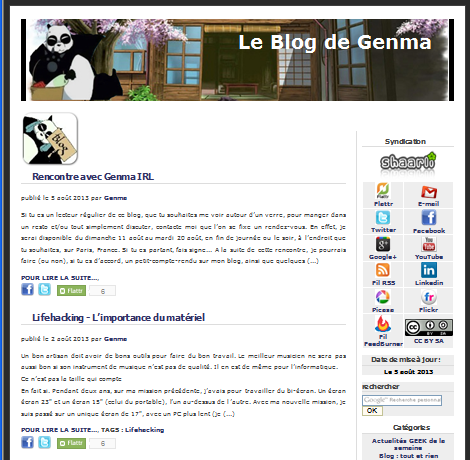
\includegraphics[width=5cm,height=5cm]{./images/blog.png} 
\end{columns}
\end{frame}

%----------------------------------------------------------------------------------------
\begin{frame}
\frametitle{Remerciements}
Parinux et tous les bénévoles du Premier-samedi. 
\\
\begin{center}
\includegraphics[scale=0.4]{./images/Logo-parignux-bleu-rouge.png}
\end{center}
Ainsi qu'à vous ici présents ;-)
\end{frame}

%----------------------------------------------------------------------------------------
\begin{frame}
\begin{center}
\Huge{Introduction}

\end{center}
\end{frame}


%----------------------------------------------------------------------------------------
\begin{frame}
\frametitle{A.I.\up{2} Apprenons l'Informatique, Apprenons Internet}

\begin{block}{Le concept d'A.I.\up{2}}
\begin{itemize}
\justifying{
\item L’Informatique et Internet sont partout dans nos vies quotidiennes. 
\item Tout à chacun soit à même de s’approprier les connaissances nécessaires et suffisantes pour comprendre ces outils qui changent les fondements mêmes de notre société, dans notre accès à l’information, aux connaissances, au partage, à la communication...
}
\end{itemize}
\end{block}
\end{frame}

%----------------------------------------------------------------------------------------
\begin{frame}
\frametitle{De quoi allons-nous parler? \\De quoi pouvons-nous parler?}
\begin{itemize}
\justifying{
\item Est-il possible d'avoir une vie privée sur Internet?
\item Qu'en est-il de nos données personnelles? 
\item On me parle d'espionnage, c'est quoi? 
}
\end{itemize}
\justifying{
Découvrons tout ça ensemble, essayons d'avoir une réponse à toutes ces questions, de façon simple et accessible.
}
\end{frame}

%----------------------------------------------------------------------------------------
\begin{frame}
\frametitle{Comment ça va se passer?}
\justifying{
Différents thèmes vont être abordés et nous reviendrons ensuite sur chacun d'eux via les questions/réponses.}
\end{frame}


%----------------------------------------------------------------------------------------
\begin{frame}
\begin{center}
\Huge{Internet, quels principes}
\end{center}
\end{frame}

%----------------------------------------------------------------------------------------
\begin{frame}
\frametitle{Internet, un réseau de réseau}
\begin{itemize}
\item Internet c'est un réseau de réseau d'ordinateurs connectés entre eux.
\item Il y a les serveurs, des gros ordinateurs, sur lesquels il y a des sites Internet.
\item Il y a des routeurs, qui servent à transmettre les colis que l'on appelle "des paquets". 
\end{itemize}
\end{frame}
%----------------------------------------------------------------------------------------
\begin{frame}
\frametitle{Le Cloud, qu'est ce que c'est?}
\begin{block}{Définition simple et pourtant vraie}
Le cloud, c'est l'ordinateur des autres.
\end{block}
\begin{center}

\includegraphics[scale=0.4]{./images/cloud.png}
\end{center}
\end{frame}
%----------------------------------------------------------------------------------------
\begin{frame}
\begin{center}
\Huge{Quels sont les problèmes?}
\end{center}
\end{frame}
%----------------------------------------------------------------------------------------
\begin{frame}
\frametitle{Les GAFAM}
GAFAM : Google, Apple, Facebook, Amazon, Microsoft
\begin{itemize}
\item Concentration des acteurs d’Internet autour de sillos;
\item Une centralisation nuisible (frein à l'innovation);
\item  Les utilisateurs de ces services derniers ne contrôlent plus leur vie numérique.
\end{itemize}
\end{frame}

%----------------------------------------------------------------------------------------
\begin{frame}
\begin{center}
\Huge{Toutes ces informations \\ que l'on donne... }
\Huge{Volontairement...}
\Huge{ou pas}
\end{center}
\end{frame}

%------------------------------------------------
\begin{frame}
\frametitle{Rien qu'avec les services Google}
\begin{itemize}
\justifying{
\item Google Search
\item GMail 
\item Google Analytics 
\item Google Maps 
\item Smartphone Android 
\item Google Calendar 
\item Google Wallet 
\item Google Docs et Drive 
\item Google Chrome, navigateur 
\item Google Photos 
\item Youtube 
\item ...
}
\end{itemize}
\end{frame}

%----------------------------------------------------------------------------------------
\begin{frame}
\frametitle{Le tracking publicitaire}
\begin{block}{Le pistage sur Internet}
\begin{itemize}
\justifying{
\item Le pistage est un terme qui comprend des méthodes aussi nombreuses et variées que les sites web, les annonceurs et d'autres utilisent pour connaître vos habitudes de navigation sur le Web. 
\item Cela comprend des informations sur les sites que vous visitez, les choses que vous aimez, n'aimez pas et achetez. 
\item Ils utilisent souvent ces données pour afficher des pubs, des produits ou services spécialement ciblés pour vous. 
}
\end{itemize}
\end{block}
\end{frame}

%----------------------------------------------------------------------------------------
\begin{frame}
\frametitle{Les réseaux sociaux}
\begin{block}{Les données que l'on donne}
\begin{itemize}
\item En remplissant sa fiche Facebook
\item En commentant, en cliquant sur J'aime...
\end{itemize}
\end{block}

\begin{block}{Les données qui sont prises à notre insu}
\begin{itemize}
\justifying{
\item Chaque bouton de partage sur les réseaux sociaux (J'aime etc.) informe le site associé que l'on a consulté tel ou tel site.
\item Les sites associés ont donc une copie de notre historique de consultation de sites Internets (et ce même en mode Navigation privée).
}
\end{itemize}
\end{block}
\end{frame}

%----------------------------------------------------------------------------------------
\begin{frame}
\frametitle{L'espionnage}

\begin{center}
\includegraphics[scale=0.4]{./images/snowden.png}
\end{center}
\begin{itemize}
\item Snowden et ses révélations (NSA)
\item La loi Renseignement en France...
\end{itemize}
\end{frame}

%----------------------------------------------------------------------------------------
\begin{frame}
\frametitle{Rappel}
\begin{center}
\Huge{Sur Internet, si c'est gratuit, c'est vous le produit }
\end{center}
\end{frame}
%----------------------------------------------------------------------------------------

%----------------------------------------------------------------------------------------
\begin{frame}
\begin{center}
\Huge{Quelles sont les solutions?}
\end{center}
\end{frame}
%----------------------------------------------------------------------------------------

%----------------------------------------------------------------------------------------
\begin{frame}
\begin{center}
\Huge{... car il y en a}
\end{center}
\end{frame}
%----------------------------------------------------------------------------------------

%----------------------------------------------------------------------------------------
\begin{frame}
\frametitle{Le logiciel libre (avec Parinux)}
\begin{itemize}
\item Passer ses ordinateurs sous un système d'exploitation (O.S.) libre. Ubuntu ou autre...
\end{itemize}
Ca tombe bien, il y a le "Premier samedi".
\end{frame}

%----------------------------------------------------------------------------------------
\begin{frame}
\frametitle{Les extensions pour Firefox}
\begin{itemize}
\item Bloquer les pubs
\item Bloquer les trackers
\item Autre...
\end{itemize}
Renseignez-vous sur ces extensions, leurs fonctions etc.
\end{frame}
%----------------------------------------------------------------------------------------
\begin{frame}
\frametitle{Dégooglisons par Framasoft}
\begin{itemize}
\item Utiliser les services fournis par Framasoft.
\end{itemize}
\end{frame}

%----------------------------------------------------------------------------------------
\begin{frame}
\begin{center}
\Huge{Aller plus loin?}
\end{center}
\end{frame}
%----------------------------------------------------------------------------------------

%----------------------------------------------------------------------------------------
\begin{frame}
\begin{center}
\Huge{Utilisez Internet, renseignez vous, cherchez, apprenez...}
\end{center}
\end{frame}
%----------------------------------------------------------------------------------------


%----------------------------------------------------------------------------------------
\begin{frame}
\begin{center}
\Huge{Et maintenant, place aux questions et discutons tous ensemble ;-)}
\end{center}
\end{frame}
%----------------------------------------------------------------------------------------
\end{document}